\documentclass[preview]{standalone}

\usepackage{amsmath}
\usepackage{amssymb}
\usepackage{parskip}
\usepackage{fullpage}
\usepackage{hyperref}
\usepackage{tikz}
\usepackage{stellar}
\usepackage{definitions}
\usepackage{bettelini}

\begin{document}

\id{limits}
\genpage

\section{Definition}

\begin{snippet}{limits-expl1}
    A limit is used to describe the behavior of a \function as its argument approaches a given value.
    The limit towards a certain value \(c\) within a \function can be be approached both from the right and from the left.
    The limit in a general sense exists if the value approached from both sides is the same and well-defined.
\end{snippet}

\begin{snippetdefinition}{extended-real-accumulation-point-definition}{Accumulation point in the extended reals}
    [\{
        "generalizations": ["accumulation-point-definition"]
    \}]
    Let \(E\subseteq \realnumbers\) and \(\xi \in \extendedrealnumbers\). Then, \(\xi\) is an \emph{extended accumulation point} of \(E\)
    if \(\xi \in \realnumbers\) and it is an \accumulationpoint of \(E\) or
    if \(\xi = \pm\infty\) and \(E\) is not \bounded above/below.
\end{snippetdefinition}

\plain{An extended accumulation point is a point for which there exist a sequence that converges to it.}

\begin{snippetdefinition}{real-function-limits-definition}{Limit of a real function}
    Let \(f \colon E \subseteq \realnumbers \fromto \realnumbers\) be a \function, \(\mu,\xi \in \extendedrealnumbers\)
    where \(\xi\) is an extended accumulation point of \(E\). Then, we write
    \[
        \lim_{x \to \xi} f(x) = \mu
    \]
    if for every \neighborhood \(I\) of \(\mu\) there exist a \neighborhood \(J\) of \(\xi\) such that
    \[
        \forall x \in (J \intersection E) \difference \{\xi\} \implies f(x) \in I
    \]
    \emph{Syntax:} we also write \(f(x) \to \mu\) as \(x\tendsto\xi\).
\end{snippetdefinition}

\begin{snippet}{limit-neighborhood-forms}
    Specification of the intervals:
    \begin{itemize}
        \item If \(\mu \in \realnumbers\), then \(I\) has form \((\mu - \varepsilon, \mu + \varepsilon)\) for some \(\varepsilon > 0\).
        \item If \(\mu = \pm\infty\), then \(I\) has form \((-\infty, M)\) or \((M, +\infty)\) for some \(M \in \realnumbers\).
        \item If \(\xi \in \realnumbers\), then \(J\) has form \((\xi - \delta, \xi + \delta)\) for some \(\delta > 0\).
        \item If \(\xi = \pm\infty\), then \(J\) has form \((-\infty, M)\) or \((M, +\infty)\) for some \(M \in \realnumbers\).
    \end{itemize}
\end{snippet}

\begin{snippet}{limits-definition-illustration}
    \begin{center}
        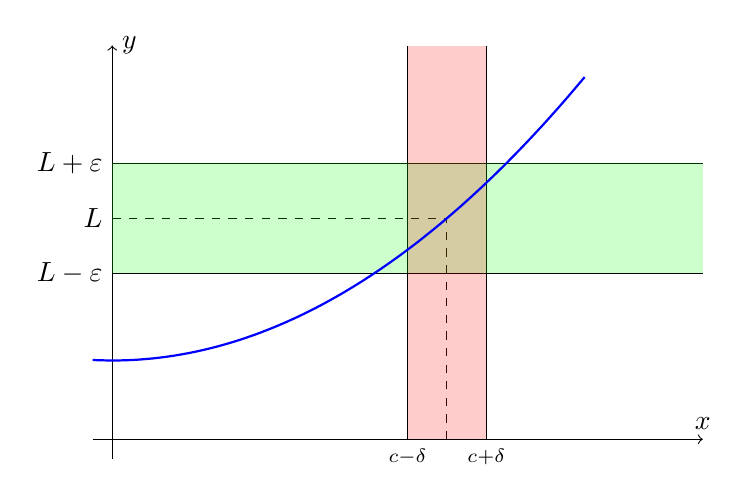
\begin{tikzpicture}[
            declare function={
                func(\x) = \x*\x / 10 + 1;
                LimX=4.25;
                Epsilon=0.7;
                Delta=0.5;
                LimY={func(LimX)};
                Width=7.5;
                Height=5;
            }
        ]
            \draw[->] (0, -0.25) -- (0, Height) node[right] {\(y\)};
            \draw[->] (-0.25, 0) -- (Width, 0) node[above] {\(x\)};

            \draw[-, dashed] (LimX, 0) -- (LimX, LimY);
            \draw[-, dashed] (0, LimY) node[left] {\(L\)} -- (LimX, LimY);

            \draw[-] (0, {LimY + Epsilon}) node[left] {\(L + \varepsilon\)} -- (Width, {LimY + Epsilon});
            \draw[-] (0, {LimY - Epsilon}) node[left] {\(L - \varepsilon\)} -- (Width, {LimY - Epsilon});

            \draw[-] ({LimX - Delta}, 0) node[below] {\(\scriptstyle c - \delta\)} -- ({LimX - Delta}, Height);
            \draw[-] ({LimX + Delta}, 0) node[below] {\(\scriptstyle c + \delta\)} -- ({LimX + Delta}, Height);

            \fill [green, opacity=0.2] (0,{LimY - Epsilon}) rectangle (Width, {LimY + Epsilon});
            \fill [red, opacity=0.2] ({LimX - Delta}, 0) rectangle ({LimX + Delta}, Height);
    
            \draw[domain=-0.25:6, smooth, variable=\x, blue, thick] plot ({\x}, {func(\x)});
        \end{tikzpicture}
    \end{center}
\end{snippet}

\begin{snippet}{limits-expl2}
    This means that for any \(x\) in the red region \(0<|x-c|<\delta\text{ or }|x-c|\in (0; \delta)\),
    the function at that point will lie in the yellow region.
    This value is closer to \(L\) than either \(L + \varepsilon\) or \(L - \varepsilon\)
    \[
        |f(x) - L| < \varepsilon
    \]
    Notice that this defintion does not require \(f\) to be defined at \(c\), but rather just around \(c\).

    We can also use this definition for limits from the right and from the left.

    The right-hand limit \(L=\lim_{x\to c^{+}}f(x)\) exists if for any arbitrary small \(\varepsilon > 0\)
    there is some \(\delta > 0\) such that
    \[
        |f(x)-L|<\varepsilon \text{ when } 0 < x-c < \delta
    \]

    The left-hand limit \(L=\lim_{x\to c^{-}}f(x)\) exists if for any arbitrary small \(\varepsilon > 0\)
    there is some \(\delta > 0\) such that
    \[
        |f(x)-L|<\varepsilon \text{ when } -\delta < x-c < 0
    \]
\end{snippet}

\begin{snippet}{limit-to-inf-convergence-illustration}
    \begin{center}
        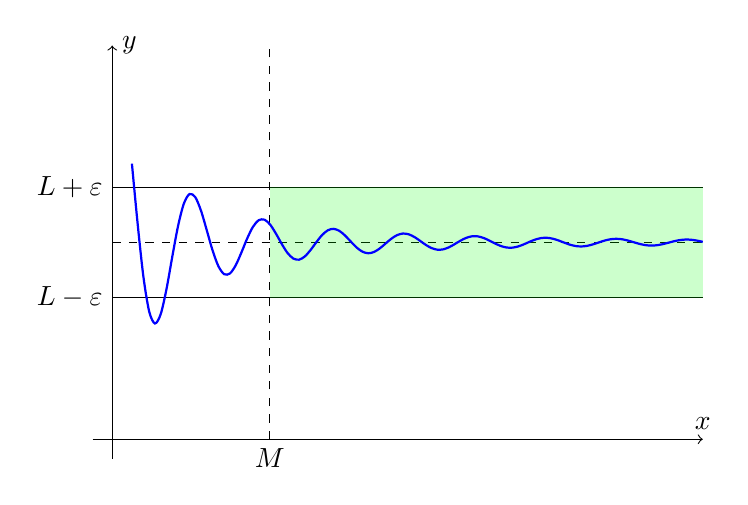
\begin{tikzpicture}[
            declare function={
                L=2.5;
                M=2;
                func(\x) = sin(7 * (\x + 1) r) / (0.4 * (\x + 1) * (\x + 1)) + L;
                Epsilon=0.7;
                Width=7.5;
                Height=5;
            }
        ]
            \draw[->] (0, -0.25) -- (0, Height) node[right] {\(y\)};
            \draw[->] (-0.25, 0) -- (Width, 0) node[above] {\(x\)};
            
            \draw[-, dashed] (0, L) -- (Width, L);
            \draw[-, dashed] (M, 0) node[below] {\(M\)} -- (M, Height);
            
            \draw[-, thin] (0, {L + Epsilon}) node[left] {\(L + \varepsilon\)} -- (Width, {L + Epsilon});
            \draw[-, thin] (0, {L - Epsilon}) node[left] {\(L - \varepsilon\)} -- (Width, {L - Epsilon});
            
            \fill [green, opacity=0.2] (M,{L - Epsilon}) rectangle (Width, {L + Epsilon});
            
            \draw[domain=0.25:Width, samples=100, smooth, variable=\x, blue, thick] plot ({\x}, {func(\x)});
        \end{tikzpicture}
    \end{center}
\end{snippet}

\begin{snippetdefinition}{real-function-right-left-limits-definition}{Right and left limits of a real function}
    Let \(f \colon E \subseteq \realnumbers \fromto \realnumbers\) be a \function, \(\mu \in \extendedrealnumbers\)
    and \(\xi\in\realnumbers\) be an \accumulationpoint of \(E\).
    Then, we write
    \[
        \lim_{x \to \xi^{-}} f(x) = \mu
        \iff
        \forall \varepsilon > 0, \exists \delta > 0 \suchthat
        \forall x \in E, \xi - \delta < x < \xi \implies \mu \leq f(x) < \mu + \varepsilon
    \]
    and
    \[
        \lim_{x \to \xi^{+}} f(x) = \mu
        \iff
        \forall \varepsilon > 0, \exists \delta > 0 \suchthat
        \forall x \in E, \xi < x < \xi + \delta \implies \mu - \varepsilon < f(x) \leq \mu
    \]
    \emph{Syntax:} we also write \(f(x) \to \mu^{\pm}\) as \(x\tendsto\xi^{\pm}\).
\end{snippetdefinition}

\plain{A limit exists if and only if the left-hand limit and the right-hand limit exist and are equal.}

\section{Results}

\plain{The following theorem acts as a bridge to allow us to use the propositions around limits of successions as
limits of functions.}

\begin{snippettheorem}{limit-of-sequence-function-bridge-theorem}{}
    Let \(f\colon E \subseteq \realnumbers \fromto \realnumbers\) and let \(\xi,\mu \in \extendedrealnumbers\)
    where \(\xi\) is an extended accumulation point of \(E\).
    Then, the following statements are equivalent:
    \begin{enumerate}
        \item \[
            \lim_{x \to \xi} f(x) = \mu
        \]
        \item \[
            \forall \{x_n\} \subseteq E \suchthat
            \forall n \in \naturalnumbers, x_n \neq \xi, x_n \tendsto \xi
            \implies f(x_n) \tendsto \mu
        \]
    \end{enumerate}
\end{snippettheorem}

\begin{snippetproof}{limit-of-sequence-function-bridge-theorem-proof}{limit-of-sequence-function-bridge-theorem}{}
    \iffproof{
        Let \(I\) be a \neighborhood of \(\mu\). We want to show that \(\exists N\) such that
        \(\forall n > N\) we have \(f(x_n) \in I\).
        Since \(f(x) \to \mu\) as \(x \tendsto \xi\), there exist a \neighborhood \(J\) of \(\xi\)
        such that \(\forall x \in (J \intersection E) \difference \{\xi\}\) we have \(f(x) \in I\).
        But since \(x_n \to \xi\) and \(\forall n, x_n \neq \xi\), there exist \(N\) such that
        \(\forall n > N\) we have \(x_n \in (J \intersection E) \difference \{\xi\}\) and thus \(f(x_n) \in I\).
    }{
        We will prove the contrapositive. Let \(\xi \in \realnumbers\) such that the \neighborhood \(J\) of \(\xi\)
        have form \((\xi - \delta, \xi + \delta)\) for some \(\delta > 0\),
        and there exist a \neighborhood \(I\) of \(\mu\) such that \(\forall \delta > 0\),
        there exist \(x_\delta \in E \intersection (\xi - \delta, \xi + \delta) \difference \{\xi\}\) such that
        \(f(x_\delta) \notin I\).
        Choose \(\delta = \frac{1}{n}\) for \(n \in \naturalnumbers\).
        Then, we have a \sequence \(\{x_n\} \subseteq E\) such that \(\forall n, \exists x_n \in E\) with \(x_n \neq \xi\) where
        \[
            \xi - \frac{1}{n} < x_n < \xi + \frac{1}{n}
        \]
        such that \(f(x_n) \notin I\).
        By the squeeze theorem, \(x_n \to \xi\) with \(x_n \neq \xi\) and \(x_n \in E\), % TOODURGENT cite
        but \(\forall n, f(x_n) \notin I\) so that \(f(x_n)\) does not converge to \(\mu\).
        The cases \(\xi = \pm\infty\) are similar.
    }
\end{snippetproof}

\section{Properties}

\begin{snippetproposition}{limit-function-uniqueness}{Uniqueness of the limit}
    Let \(f\colon E \subseteq \realnumbers \fromto \realnumbers\) and let \(\xi,\mu,\lambda \in \extendedrealnumbers\)
    where \(\xi\) is an extended accumulation point of \(E\). Then,
    \[
        \lim_{x \to \xi} f(x) = \mu
        \land
        \lim_{x \to \xi} f(x) = \lambda
        \implies \mu = \lambda
    \]
\end{snippetproposition}

\begin{snippetproof}{limit-function-uniqueness-proof}{limit-function-uniqueness}{Uniqueness of the limit}
    Since \(f(x) \to \lambda\) and \(f(x) \to \mu\),
    \(\forall \{x_n\} \subseteq E \suchthat x_n\neq \xi \land x_n \to \xi\)
    we have \(f(x_n) \tendsto \lambda\) and \(f(x_n) \tendsto \mu\).
    Since the limit of a \sequence is unique, we have \(\lambda = \mu\). %TODOURGENT cite.
\end{snippetproof}

\begin{snippettheorem}{real-function-squeeze-theorem}{Squeeze Theorem}
    Let \(f,g,h\colon E \subseteq \realnumbers \fromto \realnumbers\) and let \(\xi,\mu \in \extendedrealnumbers\)
    where \(\xi\) is an extended accumulation point of \(E\). Suppose that
    \[
        \forall x \in (E \intersection J) \difference \{\xi\},
        f(x) \leq g(x) \leq h(x)
    \]
    and
    \[
        \lim_{x \to \xi} f(x) = \lim_{x \to \xi} h(x) = \mu
    \]
    Then,
    \[
        \lim_{x \to \xi} g(x) = \mu
    \]
\end{snippettheorem}

\begin{snippetproof}{real-function-squeeze-theorem-proof}{real-function-squeeze-theorem}{Squeeze Theorem}
    By the \snippetref[limit-of-sequence-function-bridge-theorem][bridge] between \function and \sequence limits,
    the thesis is equivalent to
    \[
        \forall \{x_n\} \subseteq E \suchthat x_n\neq \xi \land x_n \to \xi,
        g(x_n) \to \mu
    \]
    Let \(\{x_n\}\) be such a \sequence.
    Since \(f(x) \to \mu\), we have \(f(x_n) \to \mu\) and since \(h(x) \to \mu\), we have \(h(x_n) \to \mu\).
    Since \(\forall x \in (E \intersection J) \difference \{\xi\}, f(x) \leq g(x) \leq h(x)\),
    and since \(x_n \to \xi \land x_n \neq \xi\) it follows that there exist \(N\) such that
    \(\forall n \leq N\) we have \(x_n \in (J \intersection E) \difference \{\xi\}\) for which
    \[
        f(x_n) \leq g(x_n) \leq h(x_n)
    \]
    and by the squeeze theorem for \sequence[sequences] %TODOURGENT cite
    the thesis follows.
\end{snippetproof}

\end{document}